% ExternE impact pathway (emissions -> transport -> damages -> valuation)
% Photos are cropped from the original slide and live in photos/
\documentclass[tikz,border=4pt]{standalone}
\renewcommand\familydefault{\sfdefault}
\usetikzlibrary{shapes.arrows,positioning}
\graphicspath{{photos/}}
\begin{document}
\begin{tikzpicture}[
    hdr/.style={font=\bfseries, align=center, anchor=south},
    flow/.style={single arrow, fill=blue, draw=blue!50!black, minimum height=12mm,
                 minimum width=9mm, single arrow head extend=2mm, inner sep=0pt},
    img/.style={inner sep=0pt}
  ]
  % column 1: emissions
  \node[img] (car)   at (0, 1.6)  {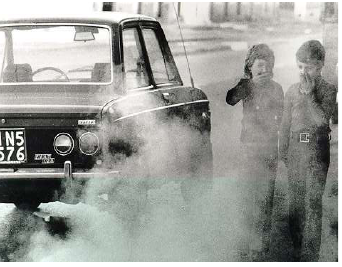
\includegraphics[width=2.6cm]{ip-car}};
  \node[img] (plant) at (0,-1.6)  {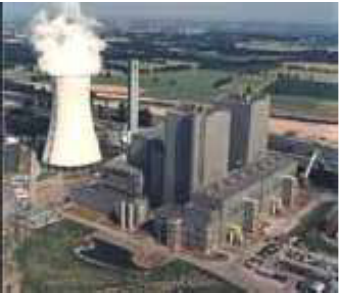
\includegraphics[width=2.6cm]{ip-powerplant}};
  % column 2: transport
  \node[img] (map)   at (4.6,0)   {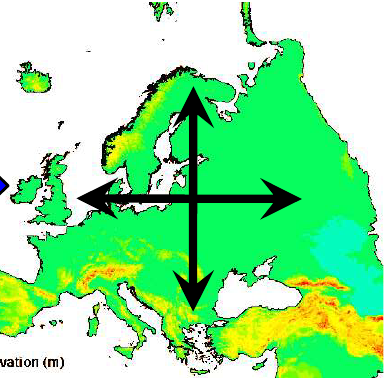
\includegraphics[width=3.4cm]{ip-transport}};
  % column 3: damages
  \node[img] (cath)  at (8.6,0)   {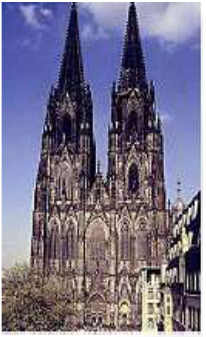
\includegraphics[width=1.6cm]{ip-cathedral}};
  \node[img, above=1mm of cath] (lungs) {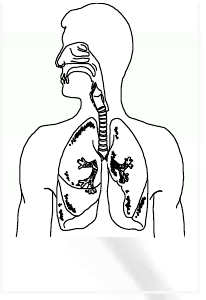
\includegraphics[width=1.6cm]{ip-lungs}};
  \node[img, below=1mm of cath] (leaf)  {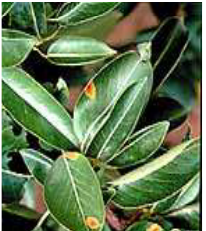
\includegraphics[width=1.6cm]{ip-leaves}};
  % column 4: valuation
  \node[img] (money) at (12.2,0)  {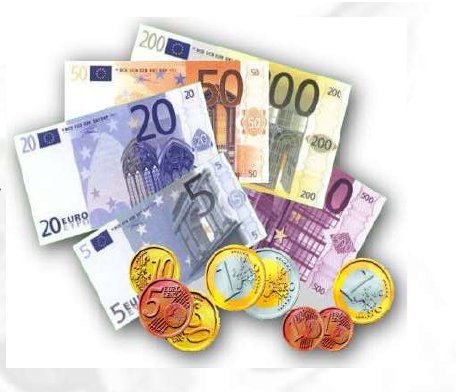
\includegraphics[width=3cm]{ip-money}};
  % arrows
  \node[flow] at (2.05,0) {};
  \node[flow] at (7.05,0) {};
  \node[flow] at (10.0,0) {};
  % headers
  \coordinate (h) at ([yshift=2mm]lungs.north);
  \node[hdr] at (0,0 |- h)    {Emissions};
  \node[hdr] at (4.6,0 |- h)  {Transport and\\chemical transformation};
  \node[hdr] at (8.6,0 |- h)  {Damages};
  \node[hdr] at (12.2,0 |- h) {Valuation};
\end{tikzpicture}
\end{document}
